\documentclass[11pt,a4paper]{article}
\usepackage[utf8]{inputenc}
\usepackage[T1]{fontenc}
\usepackage[brazil]{babel}
\usepackage{lmodern}
\usepackage{amsmath,amssymb,bm}
\usepackage{graphicx,booktabs,float,geometry,url,array,xcolor,caption}
\usepackage[hidelinks]{hyperref}
\geometry{margin=2.2cm}
\captionsetup{font=small}
\emergencystretch=2em
\providecommand{\versao}{sem versão}
% gerado por gera_dados.py; nao edite
\newcommand{\nCasos}{26}
\newcommand{\nZdois}{20}
\newcommand{\nZum}{14}
\newcommand{\casosFora}{covk=0 (2{,}1), s=400 ($-$4{,}0), alfa=2 (2{,}0), alfa=3 (3{,}5), alfa=4 (4{,}9), alfa=5 (5{,}4)}
\newcommand{\nMCmin}{170}
\newcommand{\nMCmax}{175}
\newcommand{\nMCtot}{4484}
\newcommand{\nFORMtot}{107}
\newcommand{\nLStot}{13225}
\newcommand{\nTot}{17816}
\newcommand{\linhasMin}{53}
\newcommand{\linhasMax}{600}
\newcommand{\anLSmin}{110}
\newcommand{\anLSmax}{1642}
\newcommand{\anPorLinha}{2{,}37}
\newcommand{\nLinhasMax}{3}
\newcommand{\formIt}{4{,}1}
\newcommand{\formAnMin}{3}
\newcommand{\formAnMax}{7}
\newcommand{\gdetRef}{1{,}3511}
\newcommand{\pfLSref}{11{,}52}
\newcommand{\cvLSref}{4{,}6}
\newcommand{\pfFORMref}{12{,}48}
\newcommand{\betaFORMref}{1{,}152}
\newcommand{\pfMCref}{9{,}14}
\newcommand{\nfMCref}{16}
\newcommand{\nMCref}{175}
\newcommand{\muMCref}{1{,}373}
\newcommand{\cvMCref}{24{,}5}
\newcommand{\pfAntigaRef}{9{,}36}
\newcommand{\nSpearman}{175}
\newcommand{\pfLSAlfaII}{4{,}42}
\newcommand{\pfFORMAlfaII}{4{,}12}
\newcommand{\pfCAlfaII}{3{,}90}
\newcommand{\zAlfaII}{2{,}0}
\newcommand{\cvLSAlfaII}{4{,}9}
\newcommand{\cvMCAlfaII}{26{,}1}
\newcommand{\gdetAlfaII}{1{,}5518}
\newcommand{\pfLSAlfaIII}{2{,}31}
\newcommand{\pfFORMAlfaIII}{1{,}86}
\newcommand{\pfCAlfaIII}{1{,}83}
\newcommand{\zAlfaIII}{3{,}5}
\newcommand{\cvLSAlfaIII}{4{,}9}
\newcommand{\cvMCAlfaIII}{27{,}4}
\newcommand{\gdetAlfaIII}{1{,}6921}
\newcommand{\pfLSAlfaIV}{1{,}42}
\newcommand{\pfFORMAlfaIV}{1{,}01}
\newcommand{\pfCAlfaIV}{1{,}00}
\newcommand{\zAlfaIV}{4{,}9}
\newcommand{\cvLSAlfaIV}{5{,}0}
\newcommand{\cvMCAlfaIV}{28{,}3}
\newcommand{\gdetAlfaIV}{1{,}7992}
\newcommand{\pfLSAlfaV}{0{,}97}
\newcommand{\pfFORMAlfaV}{0{,}62}
\newcommand{\pfCAlfaV}{0{,}63}
\newcommand{\zAlfaV}{5{,}4}
\newcommand{\cvLSAlfaV}{5{,}7}
\newcommand{\cvMCAlfaV}{29{,}0}
\newcommand{\gdetAlfaV}{1{,}8845}
\newcommand{\pfLSSCD}{20{,}16}
\newcommand{\pfFORMSCD}{20{,}64}
\newcommand{\pfCSCD}{21{,}93}
\newcommand{\zSCD}{$-$4{,}0}
\newcommand{\cvLSSCD}{0{,}8}
\newcommand{\cvMCSCD}{31{,}2}
\newcommand{\gdetSCD}{1{,}3511}
\newcommand{\pfLSCovkZero}{12{,}10}
\newcommand{\pfFORMCovkZero}{12{,}48}
\newcommand{\pfCCovkZero}{11{,}21}
\newcommand{\zCovkZero}{2{,}1}
\newcommand{\cvLSCovkZero}{2{,}3}
\newcommand{\cvMCCovkZero}{22{,}7}
\newcommand{\gdetCovkZero}{1{,}3511}
\newcommand{\pfLSCovcUm}{0{,}48}
\newcommand{\pfFORMCovcUm}{0{,}17}
\newcommand{\pfCCovcUm}{0{,}45}
\newcommand{\zCovcUm}{0{,}6}
\newcommand{\cvLSCovcUm}{9{,}0}
\newcommand{\cvMCCovcUm}{14{,}9}
\newcommand{\gdetCovcUm}{1{,}3511}
\newcommand{\pfLSHwIX}{13{,}90}
\newcommand{\pfFORMHwIX}{15{,}37}
\newcommand{\pfCHwIX}{12{,}58}
\newcommand{\zHwIX}{1{,}9}
\newcommand{\cvLSHwIX}{4{,}3}
\newcommand{\cvMCHwIX}{23{,}9}
\newcommand{\gdetHwIX}{1{,}3119}
\newcommand{\spc}{0{,}75}
\newcommand{\spphi}{0{,}47}
\newcommand{\spk}{0{,}35}

\title{As Seções 6.1 a 6.5 de Vargas Ceron et al.\ (2025) com a água do artigo:\\ FORM modal, line sampling e Monte
Carlo pareado, figura a figura}
\author{Diogo Cecílio}
\date{22/11/2026 --- versão \versao}
\begin{document}
\maketitle
\begin{abstract}
Os \nCasos{} casos das Seções 6.1 a 6.5 do artigo rodaram no fermi (campanha \texttt{lsCeronC}) com o MEF do NeoPZ
(fator $\Gamma$ pelo GIM) e a água do artigo: percolação permanente saturada logo depois do rebaixamento instantâneo,
com os contornos que reproduzem a Fig.~4b. Cada caso tem o FORM modal, o line sampling (LS) na direção dele, até
$CoV(P_f) = 5\,\%$, e um Monte Carlo direto pareado, ainda parcial (\nMCmin{} a \nMCmax{} de 500 realizações por caso),
que dá as densidades, a média e o $CoV$ de $\Gamma$ das figuras do artigo. Na referência, o LS dá
$P_f = \pfLSref\,\%$ ($CoV = \cvLSref\,\%$), contra $11{,}50\,\%$ do artigo. Em \nZdois{} dos \nCasos{} casos, a
diferença para o artigo fica abaixo de dois desvios. Ficam fora: \casosFora. Os desvios grandes estão na família da
anisotropia (Seção~6.4), onde crescem com $\alpha$, e no $s = 400$. O relatório de 13/11, com a água antiga, fica
superado.
\end{abstract}
\tableofcontents

\section{O que foi rodado}\label{sec:rodado}
\begin{itemize}
  \item \textbf{O problema:} o da Seção~6 do artigo~\cite{ceron2025}. Talude de $H = 5$~m a $45^\circ$, rebaixamento instantâneo do
    reservatório da crista até o pé ($h_w = H$), $c'$, $\varphi'$ e $k_v$ log-normais independentes com as médias, os
    $CoV$ e as distâncias de autocorrelação da Tabela~2 do artigo.
  \item \textbf{Três rodadas das Seções 6.1 a 6.5 até hoje:}
    \begin{enumerate}
      \item 10/11: o \texttt{SlopeRandomField} antigo (\texttt{ceron\_sat}); só as fases 1 e 3 rodaram. Os dados estão
        no backup do fermi, em \path{~/projects/runs/_arquivo/2026-11-13_backup_fermi}.
      \item 11 a 13/11: o \texttt{SlopeMonteCarlo} (a131e55), com a água permanente antiga (domínio de $25 \times
        10$~m, reservatório à direita), $\Gamma_{det} = 1{,}403$ e cerca de 5800 realizações por caso. O relatório
        figura a figura dessa rodada~\cite{antigo} está em \path{~/projects/runs/_arquivo/2026-11-11_ceron_agua_antiga/fermi_ceron/relatorio_parcial/relatorio.pdf}.
      \item 21/11 em diante: esta, com a água do artigo (\texttt{contorno=ceron}, commit 4842ae2), a mesma que o
        relatório dos contornos~\cite{contornos} (\path{Projects/PlanoDeTrabalho/contornos_agua}) mostrou reproduzir o
        $\Gamma = 1{,}336$ do artigo.
    \end{enumerate}
  \item A Tabela~\ref{tab:analises} compara as análises. As colunas ``água antiga'' das tabelas seguintes são a
    rodada 2.
\end{itemize}

\begin{table}[htbp]\centering\footnotesize\setlength{\tabcolsep}{3pt}
\caption{As análises: o artigo, a rodada de 13/11 (água antiga) e esta.}\label{tab:analises}
\begin{tabular}{p{0.13\linewidth}p{0.26\linewidth}p{0.24\linewidth}p{0.29\linewidth}}\toprule
& Ceron et al.\ (2025) & 13/11, água antiga & esta (21/11), água do artigo \\\midrule
água & percolação permanente saturada logo após o rebaixamento instantâneo (Eqs.~19 a 21) &
  permanente saturada (\texttt{TPZMatUnsaturatedUPwPa}, variante iii, \texttt{SATURADO=1}) &
  Darcy permanente saturado (\texttt{agua=sat}, \texttt{trebaix=0,0001}, \texttt{tfim=20}~h, \texttt{dt=5}~h); as
  pressões ficam congeladas no fator \\
contornos & crista, face e pé no texto; laterais e base identificados pela Fig.~4b: esquerda e base com $u = 0$,
  direita sem fluxo & $25 \times 10$~m: esquerda com a carga inicial ($u = 0$), direita com o reservatório, base
  impermeável & \texttt{contorno=ceron}: esquerda e base com $u = 0$, direita sem fluxo; domínio de $70 \times 35$~m
  (7$H$ atrás da crista, 6$H$ à frente do pé e abaixo dele) \\
fator & $\Gamma$ pela análise limite cinemática (espirais logarítmicas por trechos) & $\Gamma$ pelo GIM com
  arc-length, malha g15 com 3 níveis h & $\Gamma$ pelo GIM com arc-length, TriGMesh(1) com 5 níveis h; transiente
  na tri3 \\
$\Gamma_{det}$ & 1,336 & 1,403 & \gdetRef{} (1,340 extrapolado) \\
método & MC, $S = 10\,000$ a $90\,000$ por caso & MC, $\approx 5800$ por caso (parcial) & FORM modal + LS até
  $CoV = 5\,\%$ (30 a 600 linhas) + MC pareado (500 por caso; parcial) \\
campos & KL, $M = 2000$ & KL, $M = 2000$ (99,2\,\% da variância) & KL, $M = 2000$ (96,0\,\% da variância) \\
código & -- & a131e55 & 0d35bca \\
\bottomrule\end{tabular}\end{table}

\begin{itemize}
  \item \textbf{FORM modal:} HLRF~\cite{hasofer1974,rackwitz1978} com o gradiente modal do GIM~\cite{formulacao} (o do mecanismo de colapso), que dá zero nos termos de
    $k$ (as pressões ficam congeladas no fator). Convergiu nos \nCasos{} casos, com \formIt{} iterações em média e de
    \formAnMin{} a \formAnMax{} análises.
  \item \textbf{Line sampling~\cite{koutsourelakis2004}:} na direção do ponto de projeto, com a raiz de cada linha pelo Newton (e bisseção de
    reserva); para no primeiro $N \ge 30$ com $CoV(P_f) \le 5\,\%$, até 600 linhas. Foram de \linhasMin{} a
    \linhasMax{} linhas por caso (\anLSmin{} a \anLSmax{} análises, \anPorLinha{} por linha), sem linha perdida. Três
    casos pararam nas 600 linhas.
  \item \textbf{Monte Carlo pareado:} as mesmas realizações em todos os casos, em blocos de 5 intercalados entre os
    casos. Serve às densidades, à média e ao $CoV$ de $\Gamma$; com 500 realizações, a $P_f$ dele só é útil nos casos
    com $P_f$ acima de uns 10\,\%.
  \item \textbf{Custo até aqui:} \nTot{} análises do MEF nos \nCasos{} casos (\nFORMtot{} do FORM, \nLStot{} do LS e
    \nMCtot{} do MC). O artigo usa de 10\,000 a 90\,000 simulações por caso, com a análise limite.
\end{itemize}

\section{Determinístico (Tabelas 5 e 6)}\label{sec:det}
\begin{itemize}
  \item Com as médias, o GIM dá $\Gamma = \gdetRef$ na malha da campanha, contra $1{,}336$ do artigo. Os níveis da
    malha (1,9965; 1,6670; 1,4839; 1,4012; 1,3660; 1,3511) extrapolam para $\approx 1{,}340$: a malha da campanha
    fica $\approx 0{,}8\,\%$ acima do limite.
  \item Nas famílias $\alpha$ e $h_w/H$, o determinístico muda com o caso. Este trabalho fica de $+0{,}4$ a
    $+1{,}2\,\%$ acima do artigo em todos (Figura~\ref{fig:det}): o efeito de $\alpha$ e o mínimo em $h_w/H \approx 0{,}9$
    agora são os do artigo. Com a água antiga, $\alpha$ subia o $\Gamma$ bem menos (1,403 a 1,778, contra 1,336 a
    1,872 do artigo).
\end{itemize}
\begin{figure}[htbp]\centering
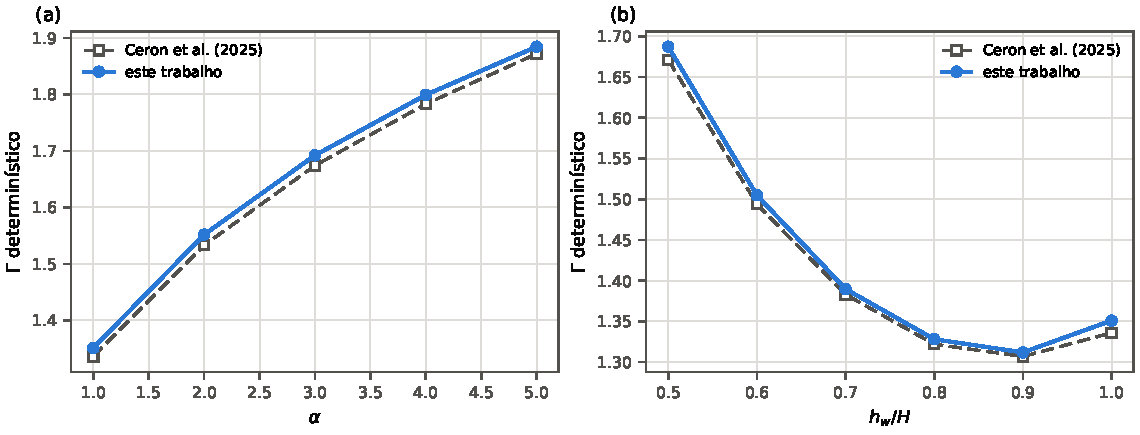
\includegraphics[width=0.8\linewidth]{figs/fig_det.pdf}
\caption{$\Gamma$ determinístico contra $\alpha$ (a) e $h_w/H$ (b): o artigo (Tabelas 5 e 6) e este trabalho.}
\label{fig:det}
\end{figure}

\clearpage
\section{Configuração de referência (Seção 6.1, Figs.~25 e 26)}\label{sec:ref}
% gerado por gera_dados.py; nao edite
\begin{table}[htbp]\centering\footnotesize
\caption{Referência (Seção 6.1). Ceron: $S = 10\,000$ simulações pela análise limite cinemática. Este trabalho: o MEF (GIM) com a água do artigo, pelo FORM modal, pelo line sampling (LS) e pelo Monte Carlo direto pareado (MC, parcial; IC exato de Clopper--Pearson~\cite{clopper1934}). Água antiga: o MC do relatório de 13/11.}\label{tab:ref}
\begin{tabular}{lrrrrr}\toprule
& Ceron & FORM modal & LS & MC & água antiga \\\midrule
$\Gamma_{det}$ & 1{,}336 & \multicolumn{3}{c}{1{,}3511} & 1{,}403 \\
$P_f$ (\%) & 11{,}50 & 12{,}48 & 11{,}52 & 12{,}00 & 9{,}36 \\
IC 95\,\% (\%) & -- & -- & [10{,}49; 12{,}56] & [9{,}28; 15{,}18] & -- \\
$CoV(P_f)$ (\%) & 2{,}77 & -- & 4{,}6 & 12{,}1 & 4{,}1 \\
$\beta$ & -- & 1{,}152 & 1{,}199 & -- & -- \\
análises do MEF & -- & 4 & 411 (173 linhas) & 500 & 5770 \\
$\mu(\Gamma)$ & 1{,}353 & -- & -- & 1{,}339 & 1{,}396 \\
$CoV(\Gamma)$ (\%) & 23{,}5 & -- & -- & 24{,}5 & 24{,}2 \\
\bottomrule\end{tabular}\end{table}

\begin{itemize}
  \item \textbf{$P_f$:} o LS dá $\pfLSref\,\%$, praticamente o número do artigo ($11{,}50\,\%$). O FORM dá
    $\pfFORMref\,\%$ ($\beta = \betaFORMref$). O MC pareado dá $\pfMCref\,\%$ (\nfMCref{} falhas em \nMCref{}), dentro
    do intervalo exato, que ainda é largo. Com a água antiga, a $P_f$ era $\pfAntigaRef\,\%$.
  \item \textbf{A distribuição de $\Gamma$:} média $\muMCref$ e $CoV = \cvMCref\,\%$ no MC, contra $1{,}353$ e
    $23{,}5\,\%$ do artigo (Figura~\ref{fig:25}a). A média fica \muDifRef\,\% da do artigo e \muVsDetRef\,\% do nosso
    determinístico; no artigo, a média fica 1,3\,\% acima do determinístico (1,353 contra 1,336). No nosso MEF, a
    variabilidade espacial baixa a média de $\Gamma$, porque o mecanismo procura as zonas fracas
    (Seção~\ref{sec:sintese}).
  \item \textbf{A malha:} a malha da campanha deixa o $\Gamma$ uns $0{,}8\,\%$ acima do limite (Seção~\ref{sec:det}).
    Pela densidade de $\Gamma$ em 1, isso baixa a $P_f$ da referência em uns 0,7 ponto: corrigida, ela ficaria perto
    de 12,2\,\%, ainda a menos de dois desvios do artigo.
\end{itemize}
\begin{figure}[htbp]\centering
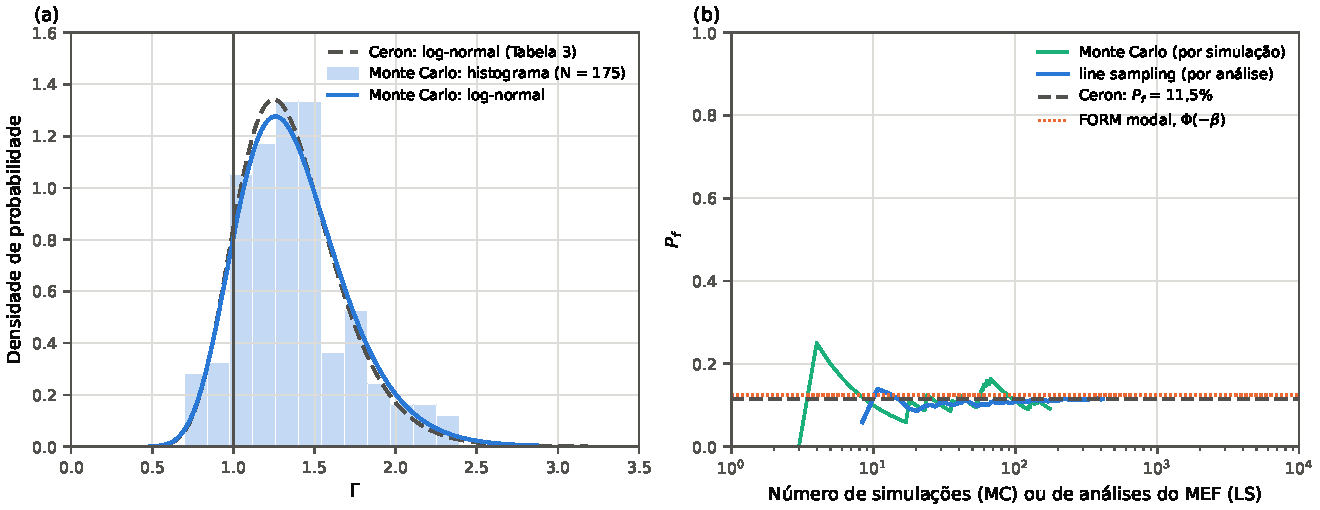
\includegraphics[width=\linewidth]{figs/fig25.pdf}
\caption{Referência. (a) Histograma do MC pareado e as log-normais (MC e artigo). (b) Convergência da $P_f$: o MC pelo
número de simulações e o LS pelo número de análises do MEF; a linha tracejada é o artigo e a pontilhada, o FORM.}
\label{fig:25}
\end{figure}

% gerado por gera_dados.py; nao edite
\begin{table}[htbp]\centering\footnotesize
\caption{Spearman parcial de 2ª ordem entre $\Gamma$ e cada variável, controlando as outras duas (Eqs.~70 e 71 do artigo), com o IC de 95\,\% (transformação de Fisher), nas 500 realizações do MC da referência. Ceron: lido nas barras da Fig.~26. Este trabalho, duas definições das variáveis de cada realização: $c'$ e $\varphi'$ médios na banda de ruptura e $k$ médio na massa que desliza; e as médias de cada campo no solo todo.}\label{tab:spearman}
\begin{tabular}{lrrr}\toprule
& Ceron (Fig.~26) & banda e massa & médias do campo \\\midrule
$k_v$ & $-$0{,}04 & 0{,}259 [0{,}18; 0{,}34] & 0{,}023 [$-$0{,}06; 0{,}11] \\
$\varphi$ & 0{,}51 & 0{,}469 [0{,}40; 0{,}53] & 0{,}067 [$-$0{,}02; 0{,}15] \\
$c$ & 0{,}88 & 0{,}771 [0{,}73; 0{,}80] & 0{,}200 [0{,}11; 0{,}28] \\
\bottomrule\end{tabular}\end{table}

\begin{itemize}
  \item \textbf{Spearman (Fig.~26):} parcial de 2ª ordem~\cite{conover1999}, como nas Eqs.~70 e~71 do artigo; com as variáveis da banda de ruptura (e o $k$ da massa que desliza), a ordem é a
    do artigo: $c$ pesa mais que $\varphi$. Com as médias do campo no solo todo, as correlações caem muito, como no
    relatório de 13/11: o que conta é o valor no mecanismo.
  \item \textbf{O $k$:} aqui ele pesa (\spk{} na massa), e no artigo quase nada ($-0{,}04$). O artigo não diz como
    define o $k$ de cada realização, então a comparação vale com cautela. Mas o sinal combina com o resto: com a água
    do artigo, um $k$ maior na massa que desliza baixa a pressão nela e sobe o $\Gamma$.
\end{itemize}
\begin{figure}[htbp]\centering
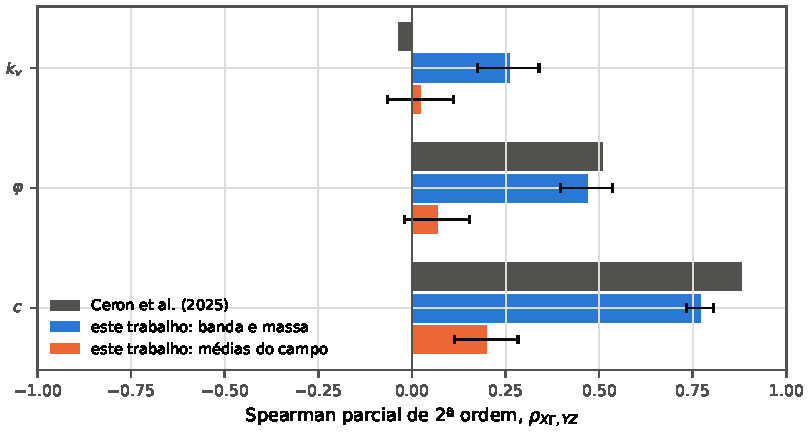
\includegraphics[width=0.62\linewidth]{figs/fig26.pdf}
\caption{Spearman parcial de 2ª ordem: o artigo (lido na Fig.~26) e este trabalho, nas duas definições das variáveis.}
\label{fig:26}
\end{figure}

\clearpage
\section{Coeficientes de variação (Seção 6.2, Figs.~27 a 30)}\label{sec:cov}
% gerado por gera_dados.py; nao edite
\begin{table}[htbp]\centering\scriptsize\setlength{\tabcolsep}{3pt}
\caption{Seção 6.2, $CoV(k_v)$: $P_f$ (\%). Ceron: Tabelas 3 a 6 do artigo, com o $CoV(P_f)$. LS: line sampling com o IC de 95\,\% e o $CoV$; $z = (P_f^{LS} - P_f^{C})/\sqrt{\sigma_{LS}^2 + \sigma_C^2}$. FORM: $\beta$ e $\Phi(-\beta)$. MC: Monte Carlo direto pareado, falhas/realizações (parcial). Água antiga: o MC do relatório de 13/11.}\label{tab:pf_covk}
\begin{tabular}{rrrrrrrrr}\toprule
$CoV(k_v)$ & Ceron & LS [IC 95\,\%] & $CoV$ & linhas/análises & $z$ & FORM: $\beta$; $P_f$ & MC & água antiga \\\midrule
0{,}0 & 11{,}21 (2{,}8) & 12{,}10 [11{,}56; 12{,}64] & 2{,}3 & 53/113 & 2{,}1 & 1{,}152; 12{,}48 & 12{,}57 (44/350) & 9{,}08 \\
0{,}6 (ref.) & 11{,}50 (2{,}8) & 11{,}52 [10{,}49; 12{,}56] & 4{,}6 & 173/411 & 0{,}0 & 1{,}152; 12{,}48 & 12{,}86 (45/350) & 9{,}36 \\
0{,}75 & 11{,}41 (2{,}8) & 11{,}70 [10{,}61; 12{,}79] & 4{,}7 & 223/541 & 0{,}5 & 1{,}152; 12{,}48 & 14{,}29 (50/350) & 9{,}44 \\
0{,}9 & 11{,}63 (2{,}8) & 12{,}18 [11{,}05; 13{,}30] & 4{,}7 & 269/662 & 0{,}8 & 1{,}152; 12{,}48 & 14{,}86 (52/350) & 9{,}60 \\
1{,}0 & 11{,}44 (2{,}8) & 12{,}12 [10{,}99; 13{,}26] & 4{,}8 & 298/731 & 1{,}0 & 1{,}152; 12{,}48 & 15{,}14 (53/350) & 9{,}74 \\
\bottomrule\end{tabular}\end{table}

% gerado por gera_dados.py; nao edite
\begin{table}[htbp]\centering\scriptsize\setlength{\tabcolsep}{3pt}
\caption{Seção 6.2, $CoV(c)$: $P_f$ (\%). Ceron: Tabelas 3 a 6 do artigo, com o $CoV(P_f)$. LS: line sampling com o IC de 95\,\% e o $CoV$; $z = (P_f^{LS} - P_f^{C})/\sqrt{\sigma_{LS}^2 + \sigma_C^2}$. FORM: $\beta$ e $\Phi(-\beta)$. MC: Monte Carlo direto pareado, falhas/realizações (parcial). Água antiga: o MC do relatório de 13/11.}\label{tab:pf_covc}
\begin{tabular}{rrrrrrrrr}\toprule
$CoV(c)$ & Ceron & LS [IC 95\,\%] & $CoV$ & linhas/análises & $z$ & FORM: $\beta$; $P_f$ & MC & água antiga \\\midrule
0{,}1 & 0{,}45 (5{,}0) & 0{,}48 [0{,}40; 0{,}57] & 9{,}0 & 600/1642 & 0{,}6 & 2{,}924; 0{,}17 & 0{,}40 (2/500) & 0{,}16 \\
0{,}3 (ref.) & 11{,}50 (2{,}8) & 11{,}52 [10{,}49; 12{,}56] & 4{,}6 & 173/411 & 0{,}0 & 1{,}152; 12{,}48 & 12{,}00 (60/500) & 9{,}36 \\
0{,}5 & 25{,}78 (1{,}7) & 26{,}36 [24{,}18; 28{,}54] & 4{,}2 & 73/160 & 0{,}5 & 0{,}540; 29{,}45 & 29{,}80 (149/500) & 24{,}47 \\
0{,}7 & 36{,}34 (1{,}3) & 39{,}15 [36{,}34; 41{,}96] & 3{,}7 & 59/135 & 1{,}9 & 0{,}214; 41{,}52 & 41{,}00 (205/500) & 37{,}45 \\
\bottomrule\end{tabular}\end{table}

% gerado por gera_dados.py; nao edite
\begin{table}[htbp]\centering\scriptsize\setlength{\tabcolsep}{3pt}
\caption{Seção 6.2, $CoV(\varphi)$: $P_f$ (\%). Ceron: Tabelas 3 a 6 do artigo, com o $CoV(P_f)$. LS: line sampling com o IC de 95\,\% e o $CoV$; $z = (P_f^{LS} - P_f^{C})/\sqrt{\sigma_{LS}^2 + \sigma_C^2}$. FORM: $\beta$ e $\Phi(-\beta)$. MC: Monte Carlo direto pareado, falhas/realizações (parcial). Água antiga: o MC do relatório de 13/11.}\label{tab:pf_covphi}
\begin{tabular}{rrrrrrrrr}\toprule
$CoV(\varphi)$ & Ceron & LS [IC 95\,\%] & $CoV$ & linhas/análises & $z$ & FORM: $\beta$; $P_f$ & MC & água antiga \\\midrule
0{,}05 & 10{,}20 (3{,}0) & 10{,}25 [9{,}30; 11{,}20] & 4{,}7 & 187/417 & 0{,}1 & 1{,}225; 11{,}02 & 11{,}59 (40/345) & 7{,}98 \\
0{,}10 (ref.) & 11{,}50 (2{,}8) & 11{,}52 [10{,}49; 12{,}56] & 4{,}6 & 173/411 & 0{,}0 & 1{,}152; 12{,}48 & 12{,}86 (45/350) & 9{,}36 \\
0{,}15 & 12{,}71 (2{,}6) & 13{,}64 [12{,}45; 14{,}83] & 4{,}5 & 160/379 & 1{,}3 & 1{,}055; 14{,}58 & 15{,}65 (54/345) & 11{,}20 \\
0{,}20 & 15{,}18 (2{,}4) & 16{,}03 [14{,}42; 17{,}65] & 5{,}1 & 122/308 & 1{,}0 & 0{,}947; 17{,}19 & 18{,}84 (65/345) & 13{,}65 \\
\bottomrule\end{tabular}\end{table}

\begin{itemize}
  \item \textbf{$P_f$:} as três famílias seguem o artigo (Figura~\ref{fig:28}). O $CoV$ de $c$ é o que mais pesa
    (de $0{,}48\,\%$ a $39\,\%$); o de $k$ quase não muda a $P_f$, como no artigo.
  \item \textbf{O FORM} erra mais onde a $P_f$ é pequena: $\pfFORMCovcUm\,\%$ contra $\pfLSCovcUm\,\%$ do LS com
    $CoV(c) = 0{,}1$. É o único caso da família com $CoV$ do LS acima de 5\,\% ($\cvLSCovcUm\,\%$, nas 600 linhas).
  \item \textbf{$CoV(k_v) = 0$:} o LS dá $\pfLSCovkZero\,\%$, contra $\pfCCovkZero\,\%$ do artigo ($z = \zCovkZero$).
    Com $k$ homogêneo, as pressões não dependem da realização, e a $P_f$ só depende de $c$ e $\varphi$.
  \item \textbf{A distribuição de $\Gamma$} (Tabelas~\ref{tab:g_covk} a \ref{tab:g_covphi}): a média fica de
    \muDifMinCovs{} a \muDifMaxCovs\,\% da do artigo. O $CoV$ acompanha o do artigo nas famílias de $k$ e de $c$, mas
    cresce mais depressa com o $CoV$ de $\varphi$ (\cvMCCovphiII{} contra 28,2\,\% com 0,2). Com $\approx \nMCmin$
    realizações, o $CoV$ amostral
    ainda depende das poucas realizações de $\Gamma$ alto, que não pesam na $P_f$: a $P_f$ desse caso bate ($z = 1{,}0$).
\end{itemize}
% gerado por gera_dados.py; nao edite
\begin{table}[htbp]\centering\scriptsize\setlength{\tabcolsep}{3pt}
\caption{Seção 6.2, $CoV(k_v)$: $\Gamma$. C: Ceron (Tabelas 3 a 6). T: este trabalho (o determinístico com as médias). MC: média e $CoV$ amostrais do Monte Carlo pareado (parcial). Antiga: o relatório de 13/11 (amostrais). $CoV$ em \%.}\label{tab:g_covk}
\begin{tabular}{rrrrrrr}\toprule
$CoV(k_v)$ & $\mu$ C & $\mu$ MC & $\mu$ antiga & $CoV$ C & $CoV$ MC & $CoV$ antiga \\\midrule
0{,}0 & 1{,}329 & 1{,}315 & 1{,}378 & 21{,}7 & 22{,}7 & 22{,}6 \\
0{,}6 (ref.) & 1{,}353 & 1{,}335 & 1{,}396 & 23{,}5 & 24{,}4 & 24{,}2 \\
0{,}75 & 1{,}375 & 1{,}345 & 1{,}403 & 24{,}8 & 25{,}2 & 24{,}9 \\
0{,}9 & 1{,}378 & 1{,}355 & 1{,}411 & 25{,}7 & 26{,}0 & 25{,}7 \\
1{,}0 & 1{,}391 & 1{,}362 & 1{,}416 & 25{,}9 & 26{,}6 & 26{,}3 \\
\bottomrule\end{tabular}\end{table}

% gerado por gera_dados.py; nao edite
\begin{table}[htbp]\centering\scriptsize\setlength{\tabcolsep}{3pt}
\caption{Seção 6.2, $CoV(c)$: $\Gamma$. C: Ceron (Tabelas 3 a 6). T: este trabalho (o determinístico com as médias). MC: média e $CoV$ amostrais do Monte Carlo pareado (parcial). Antiga: o relatório de 13/11 (amostrais). $CoV$ em \%.}\label{tab:g_covc}
\begin{tabular}{rrrrrrr}\toprule
$CoV(c)$ & $\mu$ C & $\mu$ MC & $\mu$ antiga & $CoV$ C & $CoV$ MC & $CoV$ antiga \\\midrule
0{,}1 & 1{,}367 & 1{,}361 & 1{,}418 & 13{,}2 & 14{,}3 & 13{,}8 \\
0{,}3 (ref.) & 1{,}353 & 1{,}339 & 1{,}396 & 23{,}5 & 24{,}5 & 24{,}2 \\
0{,}5 & 1{,}324 & 1{,}291 & 1{,}352 & 35{,}7 & 36{,}1 & 36{,}6 \\
0{,}7 & 1{,}296 & 1{,}220 & 1{,}290 & 47{,}9 & 47{,}5 & 48{,}5 \\
\bottomrule\end{tabular}\end{table}

% gerado por gera_dados.py; nao edite
\begin{table}[htbp]\centering\scriptsize\setlength{\tabcolsep}{3pt}
\caption{Seção 6.2, $CoV(\varphi)$: $\Gamma$. C: Ceron (Tabelas 3 a 6). T: este trabalho (o determinístico com as médias). MC: média e $CoV$ amostrais do Monte Carlo pareado (parcial). Antiga: o relatório de 13/11 (amostrais). $CoV$ em \%.}\label{tab:g_covphi}
\begin{tabular}{rrrrrrr}\toprule
$CoV(\varphi)$ & $\mu$ C & $\mu$ MC & $\mu$ antiga & $CoV$ C & $CoV$ MC & $CoV$ antiga \\\midrule
0{,}05 & 1{,}351 & 1{,}336 & 1{,}396 & 22{,}2 & 22{,}9 & 22{,}8 \\
0{,}10 (ref.) & 1{,}353 & 1{,}335 & 1{,}396 & 23{,}5 & 24{,}4 & 24{,}2 \\
0{,}15 & 1{,}357 & 1{,}337 & 1{,}397 & 25{,}5 & 27{,}2 & 26{,}6 \\
0{,}20 & 1{,}361 & 1{,}339 & 1{,}399 & 28{,}2 & 32{,}1 & 29{,}8 \\
\bottomrule\end{tabular}\end{table}

\begin{figure}[htbp]\centering
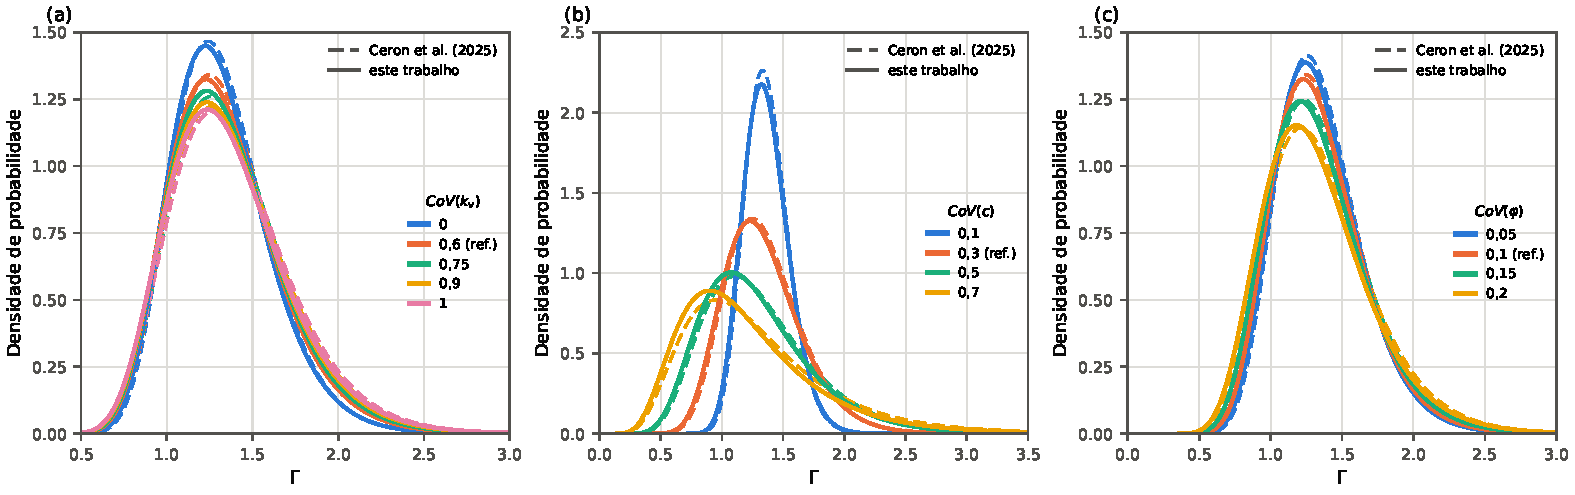
\includegraphics[width=\linewidth]{figs/fig27.pdf}
\caption{Densidades log-normais de $\Gamma$ com o $CoV$ de $k_v$ (a), $c$ (b) e $\varphi$ (c). Tracejado: o artigo;
cheio: este trabalho (MC pareado).}\label{fig:27}
\end{figure}
\begin{figure}[htbp]\centering
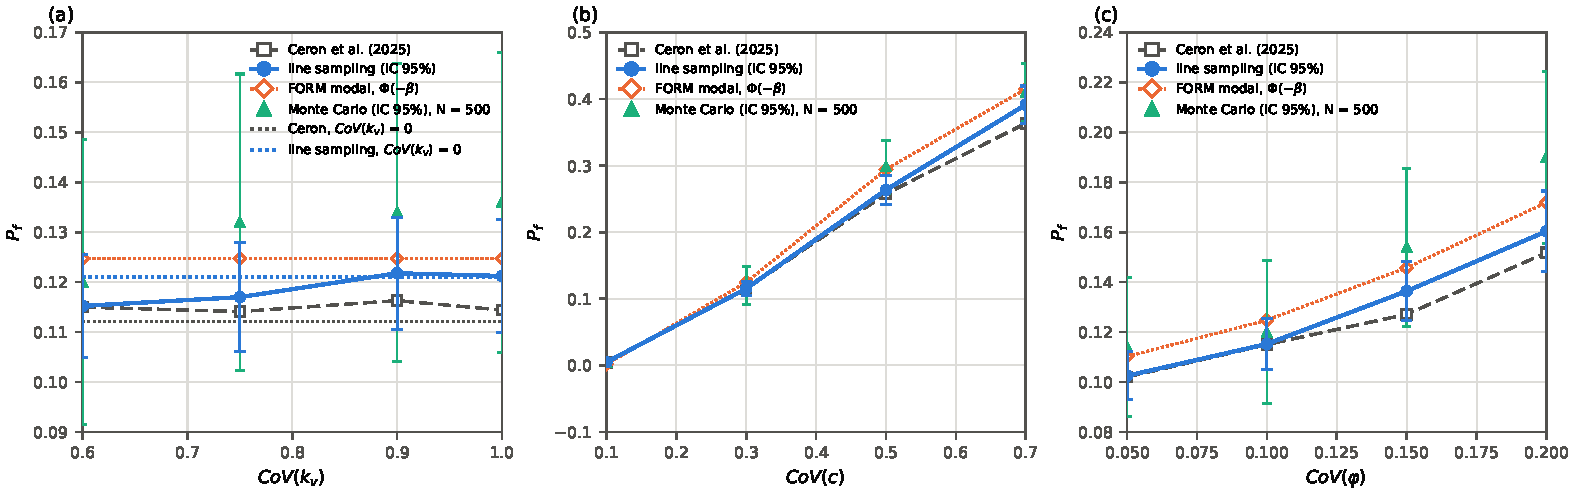
\includegraphics[width=\linewidth]{figs/fig28.pdf}
\caption{$P_f$ contra o $CoV$ de $k_v$ (a), $c$ (b) e $\varphi$ (c): o artigo, o LS (IC de 95\,\%), o FORM e o MC
pareado (IC de 95\,\%).}\label{fig:28}
\end{figure}
\begin{figure}[htbp]\centering
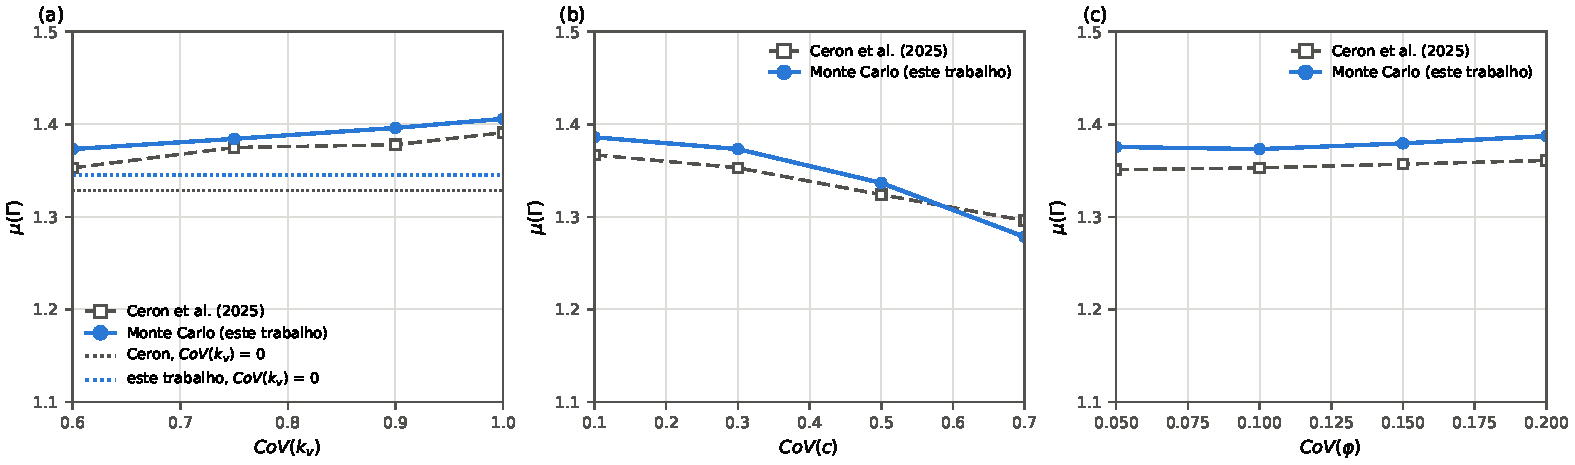
\includegraphics[width=\linewidth]{figs/fig29.pdf}
\caption{$\mu(\Gamma)$ contra o $CoV$ de $k_v$ (a), $c$ (b) e $\varphi$ (c).}\label{fig:29}
\end{figure}
\begin{figure}[htbp]\centering
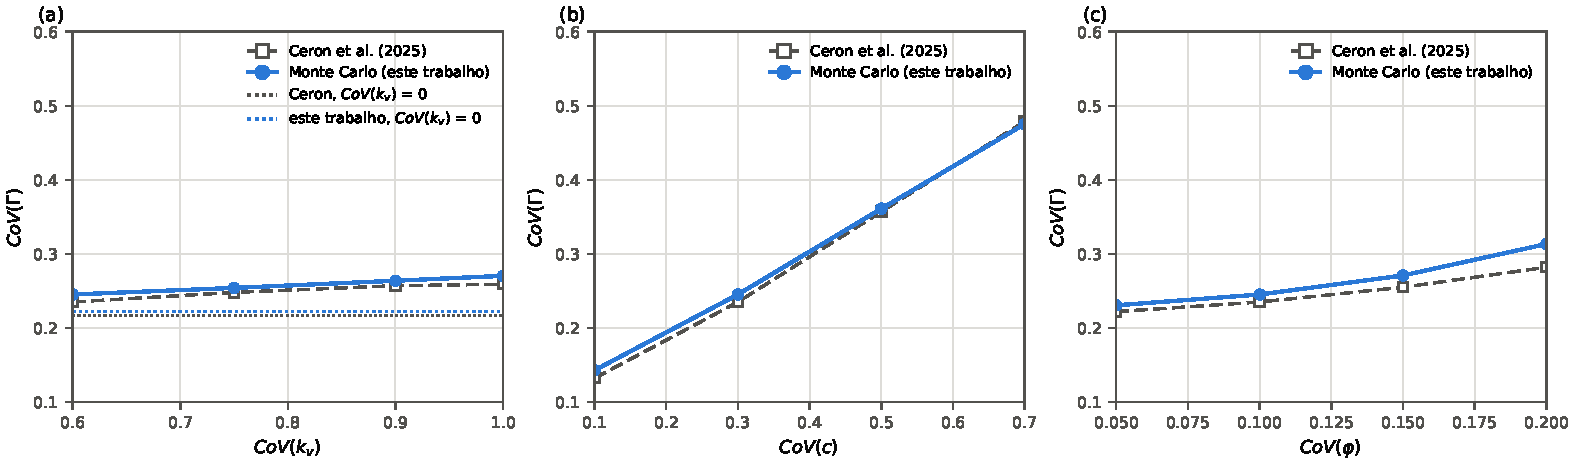
\includegraphics[width=\linewidth]{figs/fig30.pdf}
\caption{$CoV(\Gamma)$ contra o $CoV$ de $k_v$ (a), $c$ (b) e $\varphi$ (c).}\label{fig:30}
\end{figure}

\clearpage
\section{Distâncias de autocorrelação (Seção 6.3, Fig.~31)}\label{sec:s}
% gerado por gera_dados.py; nao edite
\begin{table}[htbp]\centering\scriptsize\setlength{\tabcolsep}{3pt}
\caption{Seção 6.3, $s$: $P_f$ (\%). Ceron: Tabelas 3 a 6 do artigo, com o $CoV(P_f)$. LS: line sampling com o IC de 95\,\% e o $CoV$; $z = (P_f^{LS} - P_f^{C})/\sqrt{\sigma_{LS}^2 + \sigma_C^2}$. FORM: $\beta$ e $\Phi(-\beta)$. MC: Monte Carlo direto pareado, falhas/realizações (parcial). Água antiga: o MC do relatório de 13/11.}\label{tab:pf_s}
\begin{tabular}{rrrrrrrrr}\toprule
$s$ & Ceron & LS [IC 95\,\%] & $CoV$ & linhas/análises & $z$ & FORM: $\beta$; $P_f$ & MC & água antiga \\\midrule
1 (ref.) & 11{,}50 (2{,}8) & 11{,}52 [10{,}49; 12{,}56] & 4{,}6 & 173/411 & 0{,}0 & 1{,}152; 12{,}48 & 12{,}86 (45/350) & 9{,}36 \\
1{,}5 & 13{,}94 (2{,}5) & 14{,}44 [13{,}10; 15{,}77] & 4{,}7 & 114/258 & 0{,}6 & 1{,}050; 14{,}70 & 14{,}49 (50/345) & 11{,}31 \\
2 & 14{,}99 (2{,}4) & 15{,}78 [14{,}37; 17{,}20] & 4{,}6 & 81/177 & 1{,}0 & 0{,}989; 16{,}13 & 15{,}36 (53/345) & 12{,}71 \\
5 & 18{,}93 (2{,}1) & 18{,}37 [17{,}09; 19{,}65] & 3{,}6 & 66/136 & $-$0{,}7 & 0{,}888; 18{,}72 & 20{,}29 (70/345) & 15{,}29 \\
10 & 19{,}85 (2{,}0) & 19{,}27 [18{,}12; 20{,}43] & 3{,}1 & 53/112 & $-$0{,}8 & 0{,}851; 19{,}73 & 19{,}13 (66/345) & 16{,}27 \\
20 & 20{,}23 (2{,}0) & 20{,}26 [19{,}26; 21{,}26] & 2{,}5 & 53/110 & 0{,}0 & 0{,}835; 20{,}17 & 20{,}29 (70/345) & 16{,}76 \\
400 & 21{,}93 (1{,}9) & 20{,}16 [19{,}86; 20{,}46] & 0{,}8 & 53/110 & $-$4{,}0 & 0{,}819; 20{,}64 & 19{,}42 (67/345) & 17{,}05 \\
\bottomrule\end{tabular}\end{table}

% gerado por gera_dados.py; nao edite
\begin{table}[htbp]\centering\scriptsize\setlength{\tabcolsep}{3pt}
\caption{Seção 6.3, $s$: $\Gamma$. C: Ceron (Tabelas 3 a 6). T: este trabalho (o determinístico com as médias). MC: média e $CoV$ amostrais do Monte Carlo pareado (parcial). Antiga: o relatório de 13/11 (amostrais). $CoV$ em \%.}\label{tab:g_s}
\begin{tabular}{rrrrrrr}\toprule
$s$ & $\mu$ C & $\mu$ MC & $\mu$ antiga & $CoV$ C & $CoV$ MC & $CoV$ antiga \\\midrule
1 (ref.) & 1{,}353 & 1{,}373 & 1{,}396 & 23{,}5 & 24{,}5 & 24{,}2 \\
1{,}5 & 1{,}356 & 1{,}371 & 1{,}404 & 25{,}9 & 25{,}9 & 26{,}1 \\
2 & 1{,}361 & 1{,}376 & 1{,}403 & 27{,}3 & 25{,}5 & 27{,}3 \\
5 & 1{,}350 & 1{,}383 & 1{,}405 & 29{,}9 & 30{,}7 & 29{,}6 \\
10 & 1{,}348 & 1{,}369 & 1{,}406 & 31{,}1 & 28{,}2 & 30{,}6 \\
20 & 1{,}355 & 1{,}378 & 1{,}405 & 31{,}7 & 30{,}2 & 31{,}1 \\
400 & 1{,}348 & 1{,}371 & 1{,}404 & 32{,}1 & 31{,}2 & 31{,}5 \\
\bottomrule\end{tabular}\end{table}

\begin{itemize}
  \item \textbf{$P_f$:} cresce com $s$ e satura, como no artigo. Até $s = 2$ o LS fica um pouco acima do artigo; de
    $s = 5$ em diante, igual ou um pouco abaixo.
  \item \textbf{$s = 400$} ($z = \zSCD$): os campos ficam praticamente homogêneos, e a $P_f$ vira a de duas variáveis
    ($c$ e $\varphi$): um $k$ uniforme não muda as pressões da percolação permanente. O LS dá $\pfLSSCD\,\%$ com $CoV$
    de $\cvLSSCD\,\%$, e o artigo, $\pfCSCD\,\%$. Duas causas pesam aqui mais que nos outros casos:
    \begin{itemize}
      \item a malha: os $0{,}8\,\%$ de $\Gamma$ acima do limite baixam a $P_f$ em uns 0,7 ponto, pela densidade de
        $\Gamma$ em 1, que é alta neste caso;
      \item sem variabilidade espacial, o mecanismo livre do MEF não tem caminho fraco para achar, e o efeito que puxa
        a nossa $P_f$ para cima nos outros casos some.
    \end{itemize}
    O resto da diferença ($\approx 1$ ponto) fica em aberto. Como são só duas variáveis, a $P_f$ deste caso pode ser
    calculada por integração numérica numa grade de determinísticos em $(c, \varphi)$, sem amostragem.
\end{itemize}
\begin{figure}[htbp]\centering
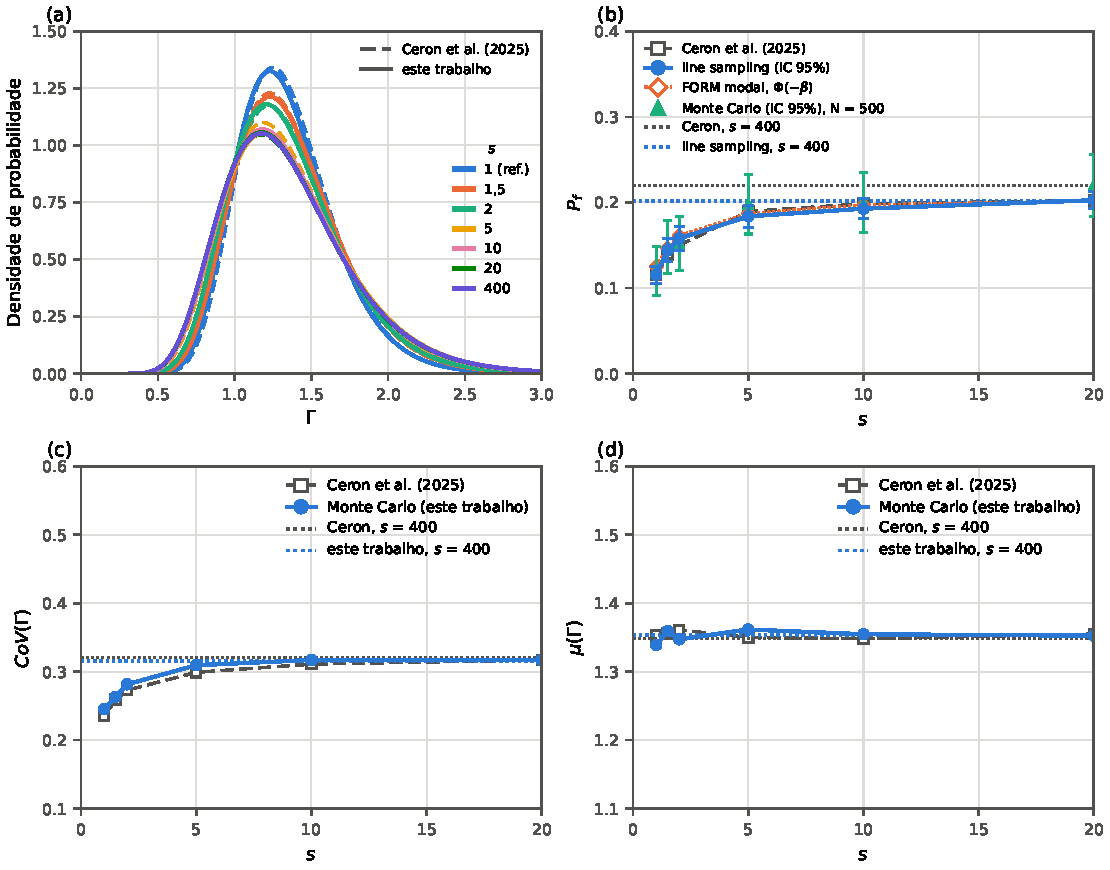
\includegraphics[width=\linewidth]{figs/fig31.pdf}
\caption{(a) Densidades log-normais de $\Gamma$; (b) $P_f$; (c) $CoV(\Gamma)$; (d) $\mu(\Gamma)$, com $s$. O caso
$s = 400$ aparece em (b) a (d) como linha horizontal, como no artigo.}\label{fig:31}
\end{figure}

\clearpage
\section{Anisotropia da permeabilidade (Seção 6.4, Fig.~32)}\label{sec:alfa}
% gerado por gera_dados.py; nao edite
\begin{table}[htbp]\centering\scriptsize\setlength{\tabcolsep}{3pt}
\caption{Seção 6.4, $\alpha$: $P_f$ (\%). Ceron: Tabelas 3 a 6 do artigo, com o $CoV(P_f)$. LS: line sampling com o IC de 95\,\% e o $CoV$; $z = (P_f^{LS} - P_f^{C})/\sqrt{\sigma_{LS}^2 + \sigma_C^2}$. FORM: $\beta$ e $\Phi(-\beta)$. MC: Monte Carlo direto pareado, falhas/realizações (parcial). Água antiga: o MC do relatório de 13/11.}\label{tab:pf_alfa}
\begin{tabular}{rrrrrrrrr}\toprule
$\alpha$ & Ceron & LS [IC 95\,\%] & $CoV$ & linhas/análises & $z$ & FORM: $\beta$; $P_f$ & MC & água antiga \\\midrule
1 (ref.) & 11{,}50 (2{,}8) & 11{,}52 [10{,}49; 12{,}56] & 4{,}6 & 173/411 & 0{,}0 & 1{,}152; 12{,}48 & 12{,}86 (45/350) & 9{,}36 \\
2 & 3{,}90 (3{,}5) & 4{,}42 [4{,}00; 4{,}84] & 4{,}9 & 310/719 & 2{,}0 & 1{,}736; 4{,}12 & 5{,}80 (20/345) & 4{,}26 \\
3 & 1{,}83 (4{,}2) & 2{,}31 [2{,}09; 2{,}54] & 4{,}9 & 463/1083 & 3{,}5 & 2{,}083; 1{,}86 & 2{,}91 (10/344) & 2{,}67 \\
4 & 1{,}00 (5{,}0) & 1{,}42 [1{,}28; 1{,}56] & 5{,}0 & 600/1449 & 4{,}9 & 2{,}321; 1{,}01 & 1{,}17 (4/343) & 1{,}85 \\
5 & 0{,}63 (4{,}7) & 0{,}97 [0{,}86; 1{,}08] & 5{,}7 & 600/1416 & 5{,}4 & 2{,}503; 0{,}62 & 0{,}87 (3/343) & 1{,}54 \\
\bottomrule\end{tabular}\end{table}

% gerado por gera_dados.py; nao edite
\begin{table}[htbp]\centering\scriptsize\setlength{\tabcolsep}{3pt}
\caption{Seção 6.4, $\alpha$: $\Gamma$. C: Ceron (Tabelas 3 a 6). T: este trabalho (o determinístico com as médias). MC: média e $CoV$ amostrais do Monte Carlo pareado (parcial). Antiga: o relatório de 13/11 (amostrais). $CoV$ em \%.}\label{tab:g_alfa}
\begin{tabular}{rrrrrrrrrr}\toprule
$\alpha$ & $\Gamma_{det}$ C & $\Gamma_{det}$ T & $\Gamma_{det}$ antiga & $\mu$ C & $\mu$ MC & $\mu$ antiga & $CoV$ C & $CoV$ MC & $CoV$ antiga \\\midrule
1 (ref.) & 1{,}336 & 1{,}351 & 1{,}403 & 1{,}353 & 1{,}335 & 1{,}396 & 23{,}5 & 24{,}4 & 24{,}2 \\
2 & 1{,}533 & 1{,}552 & 1{,}562 & 1{,}562 & 1{,}529 & 1{,}547 & 24{,}9 & 25{,}7 & 25{,}0 \\
3 & 1{,}674 & 1{,}692 & 1{,}659 & 1{,}704 & 1{,}662 & 1{,}636 & 25{,}3 & 26{,}6 & 25{,}5 \\
4 & 1{,}783 & 1{,}799 & 1{,}726 & 1{,}821 & 1{,}762 & 1{,}696 & 26{,}0 & 27{,}3 & 25{,}8 \\
5 & 1{,}872 & 1{,}884 & 1{,}778 & 1{,}910 & 1{,}839 & 1{,}738 & 26{,}4 & 27{,}9 & 26{,}1 \\
\bottomrule\end{tabular}\end{table}

\begin{itemize}
  \item \textbf{O determinístico bate; a média do MC, não tanto:} $\Gamma_{det}$ fica de +0,7 a +1,2\,\% do artigo,
    e a média do MC, de \muDifMinAlfa{} a \muDifMaxAlfa\,\%, com a diferença crescendo com $\alpha$ nos dados atuais
    (Tabela~\ref{tab:g_alfa}).
  \item \textbf{A $P_f$ não bate, e a diferença cresce com $\alpha$:} o LS dá $\pfLSAlfaII$, $\pfLSAlfaIII$,
    $\pfLSAlfaIV$ e $\pfLSAlfaV\,\%$, contra $\pfCAlfaII$, $\pfCAlfaIII$, $\pfCAlfaIV$ e $\pfCAlfaV\,\%$ do artigo
    ($z$ de \zAlfaII{} a \zAlfaV). A água antiga também dava $P_f$ acima do artigo nesta família, e mais.
  \item \textbf{O $CoV$ de $\Gamma$ é maior aqui:} no MC pareado, ele vai de $\cvMCAlfaII$ a $\cvMCAlfaV\,\%$, contra
    24,9 a 26,4\,\% do artigo, e a diferença cresce com $\alpha$. Média menor e $CoV$ maior engordam a cauda de baixo,
    que é onde fica a $P_f$ quando ela é pequena. Com \nMCmin{} realizações, o erro do $CoV$ amostral é de uns
    \cvErroPts{} ponto: o sinal é consistente nos quatro casos, mas cada um sozinho é fraco.
  \item \textbf{O FORM fica com o artigo, o LS não:} o FORM dá $\pfFORMAlfaII$, $\pfFORMAlfaIII$, $\pfFORMAlfaIV$ e
    $\pfFORMAlfaV\,\%$, quase os números do artigo. A Figura~\ref{fig:raizes} mostra por quê: as raízes das linhas
    espalham em torno do $\beta$ do FORM (de $\pm 0{,}5$), e, como $\Phi(-c)$ é convexa na cauda, a média de
    $\Phi(-c)$ fica acima de $\Phi(-\beta)$. Esse espalhamento vem das direções que o FORM não vê, entre elas o campo
    de $k$, cujo gradiente modal é zero.
  \item \textbf{A leitura provisória:} no nosso modelo, o campo de $k$ (e o resto da variabilidade fora da direção do
    FORM) espalha mais o $\Gamma$ quando $k_h > k_v$, e isso aparece na cauda. O Spearman do $k$ na referência
    (Seção~\ref{sec:ref}) vai na mesma direção. Nada indica erro na busca das raízes: as linhas levaram 2,4 análises
    em média, nenhuma ficou sem raiz e nenhuma se perdeu.
  \item \textbf{Testes que decidem:} (1) o caso $\alpha = 4$ com $CoV(k_v) = 0$: se o $z$ cair, a diferença vem do
    campo de $k$; (2) o $\Gamma$ cinemático do Ceron, refeito em Python (\path{Projects/CeronCinematico}), nas mesmas
    realizações do $\alpha = 4$, para separar o método (mecanismo imposto contra livre) da água; (3) refazer por
    bisseção as 10 linhas de menor raiz do $\alpha = 4$, que levam um quarto da $P_f$.
\end{itemize}
\begin{figure}[htbp]\centering
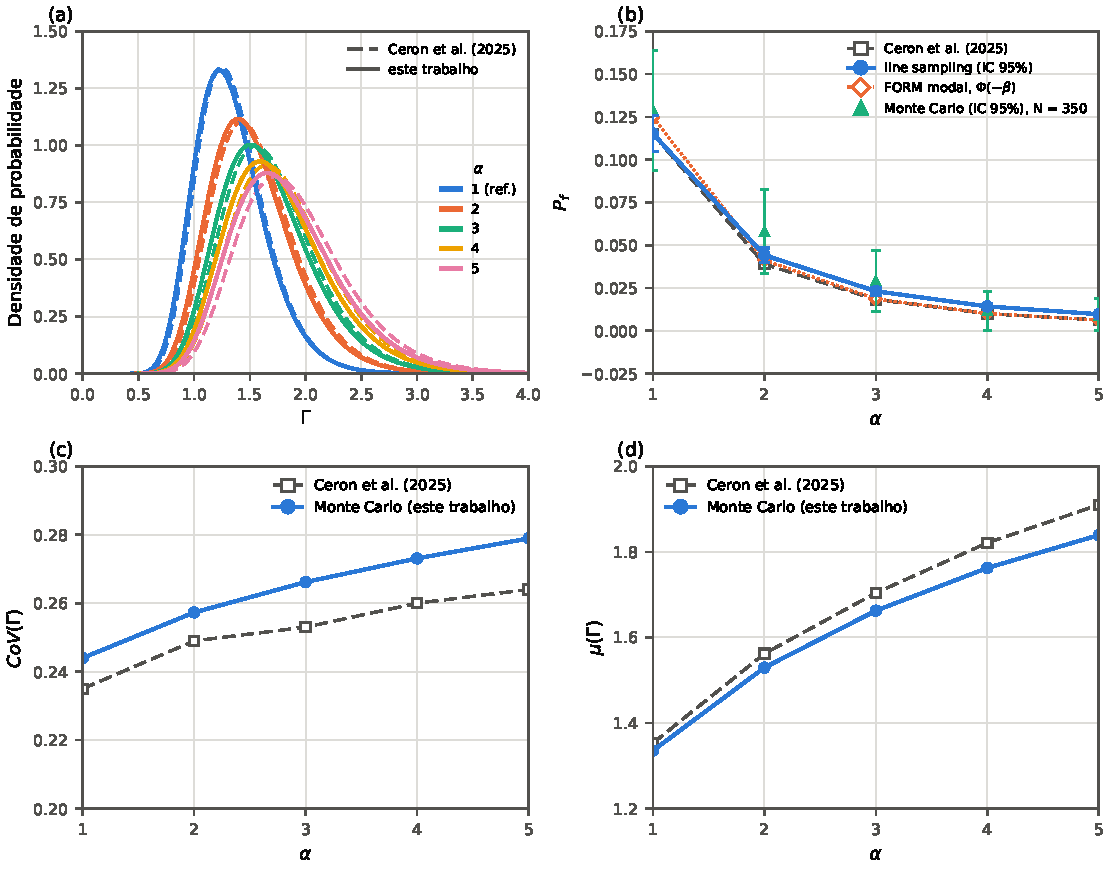
\includegraphics[width=\linewidth]{figs/fig32.pdf}
\caption{(a) Densidades log-normais de $\Gamma$; (b) $P_f$; (c) $CoV(\Gamma)$; (d) $\mu(\Gamma)$, com $\alpha$.}
\label{fig:32}
\end{figure}
\begin{figure}[htbp]\centering
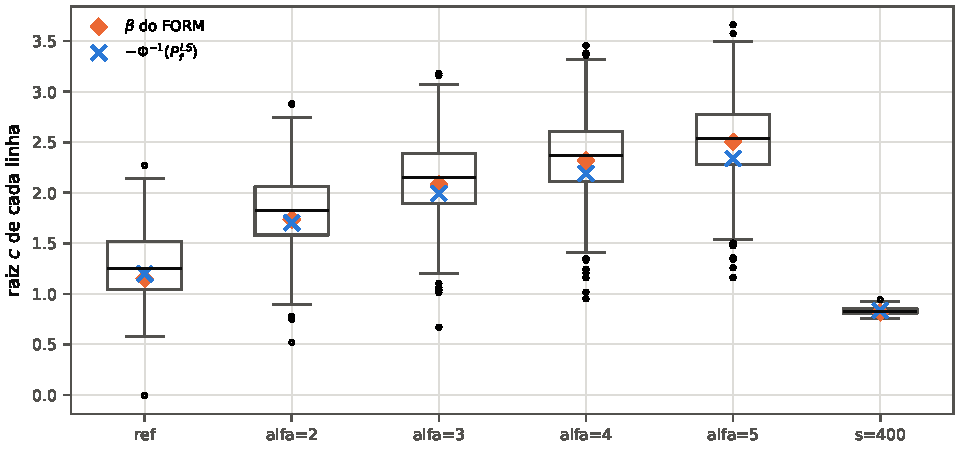
\includegraphics[width=\linewidth]{figs/fig_raizes.pdf}
\caption{As raízes $c$ das linhas do LS (caixas: quartis; bigodes: 1,5 vez a distância interquartil), o $\beta$ do FORM
e o índice equivalente do LS, $-\Phi^{-1}(P_f^{LS})$, na referência, na família $\alpha$ e em $s = 400$.}
\label{fig:raizes}
\end{figure}

\clearpage
\section{Altura do rebaixamento (Seção 6.5, Fig.~33)}\label{sec:hw}
% gerado por gera_dados.py; nao edite
\begin{table}[htbp]\centering\scriptsize\setlength{\tabcolsep}{3pt}
\caption{Seção 6.5, $h_w/H$: $P_f$ (\%). Ceron: Tabelas 3 a 6 do artigo, com o $CoV(P_f)$. LS: line sampling com o IC de 95\,\% e o $CoV$; $z = (P_f^{LS} - P_f^{C})/\sqrt{\sigma_{LS}^2 + \sigma_C^2}$. FORM: $\beta$ e $\Phi(-\beta)$. MC: Monte Carlo direto pareado, falhas/realizações (parcial). Água antiga: o MC do relatório de 13/11.}\label{tab:pf_hw}
\begin{tabular}{rrrrrrrrr}\toprule
$h_w/H$ & Ceron & LS [IC 95\,\%] & $CoV$ & linhas/análises & $z$ & FORM: $\beta$; $P_f$ & MC & água antiga \\\midrule
0{,}5 & 1{,}38 (4{,}9) & 1{,}53 [1{,}39; 1{,}67] & 4{,}8 & 307/683 & 1{,}5 & 2{,}155; 1{,}56 & 1{,}60 (8/500) & 1{,}20 \\
0{,}6 & 4{,}20 (4{,}8) & 4{,}64 [4{,}20; 5{,}09] & 4{,}9 & 199/441 & 1{,}5 & 1{,}648; 4{,}96 & 6{,}20 (31/500) & 3{,}43 \\
0{,}7 & 8{,}54 (3{,}3) & 8{,}79 [8{,}03; 9{,}56] & 4{,}4 & 159/354 & 0{,}5 & 1{,}290; 9{,}85 & 9{,}40 (47/500) & 6{,}81 \\
0{,}8 & 11{,}99 (2{,}7) & 12{,}44 [11{,}37; 13{,}52] & 4{,}4 & 145/330 & 0{,}7 & 1{,}075; 14{,}13 & 13{,}40 (67/500) & 9{,}74 \\
0{,}9 & 12{,}58 (2{,}6) & 13{,}90 [12{,}72; 15{,}08] & 4{,}3 & 152/348 & 1{,}9 & 1{,}021; 15{,}37 & 16{,}20 (81/500) & 10{,}71 \\
1{,}0 (ref.) & 11{,}50 (2{,}8) & 11{,}52 [10{,}49; 12{,}56] & 4{,}6 & 173/411 & 0{,}0 & 1{,}152; 12{,}48 & 12{,}00 (60/500) & 9{,}36 \\
\bottomrule\end{tabular}\end{table}

% gerado por gera_dados.py; nao edite
\begin{table}[htbp]\centering\scriptsize\setlength{\tabcolsep}{3pt}
\caption{Seção 6.5, $h_w/H$: $\Gamma$. C: Ceron (Tabelas 3 a 6). T: este trabalho (o determinístico com as médias). MC: média e $CoV$ amostrais do Monte Carlo pareado (parcial). Antiga: o relatório de 13/11 (amostrais). $CoV$ em \%.}\label{tab:g_hw}
\begin{tabular}{rrrrrrrrrr}\toprule
$h_w/H$ & $\Gamma_{det}$ C & $\Gamma_{det}$ T & $\Gamma_{det}$ antiga & $\mu$ C & $\mu$ MC & $\mu$ antiga & $CoV$ C & $CoV$ MC & $CoV$ antiga \\\midrule
0{,}5 & 1{,}671 & 1{,}687 & 1{,}739 & 1{,}670 & 1{,}657 & 1{,}712 & 22{,}6 & 23{,}6 & 23{,}6 \\
0{,}6 & 1{,}494 & 1{,}505 & 1{,}559 & 1{,}502 & 1{,}482 & 1{,}541 & 22{,}9 & 23{,}5 & 23{,}5 \\
0{,}7 & 1{,}383 & 1{,}390 & 1{,}447 & 1{,}393 & 1{,}372 & 1{,}435 & 22{,}5 & 23{,}5 & 23{,}5 \\
0{,}8 & 1{,}322 & 1{,}328 & 1{,}385 & 1{,}338 & 1{,}312 & 1{,}377 & 23{,}1 & 23{,}7 & 23{,}6 \\
0{,}9 & 1{,}307 & 1{,}312 & 1{,}371 & 1{,}325 & 1{,}298 & 1{,}363 & 23{,}1 & 24{,}0 & 23{,}8 \\
1{,}0 (ref.) & 1{,}336 & 1{,}351 & 1{,}403 & 1{,}353 & 1{,}335 & 1{,}396 & 23{,}5 & 24{,}4 & 24{,}2 \\
\bottomrule\end{tabular}\end{table}

\begin{itemize}
  \item \textbf{$P_f$:} os cinco casos ficam a menos de dois desvios do artigo, todos um pouco acima, e o máximo
    perto de $h_w/H = 0{,}9$ aparece como no artigo.
  \item \textbf{$\Gamma$:} o determinístico e o $CoV$ seguem o artigo; a média do MC fica de \muDifMinHw{} a \muDifMaxHw\,\% da do
    artigo.
\end{itemize}
\begin{figure}[htbp]\centering
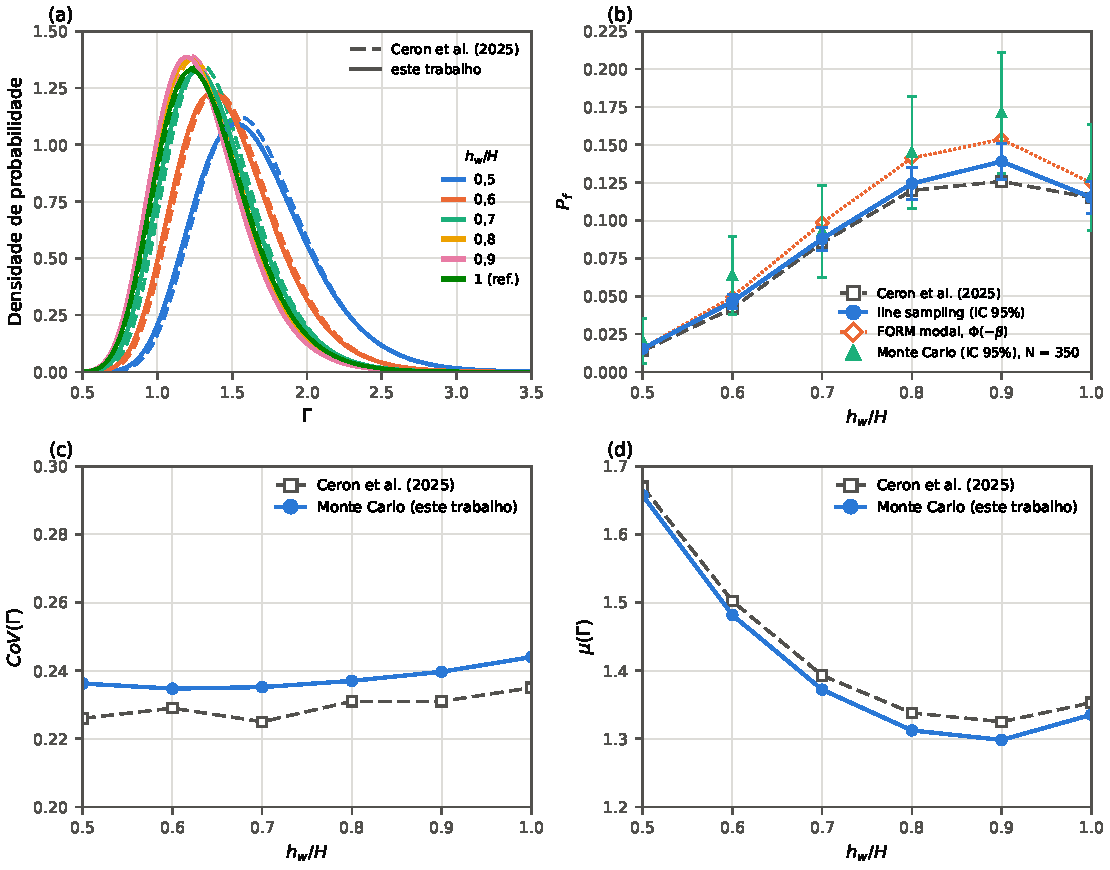
\includegraphics[width=\linewidth]{figs/fig33.pdf}
\caption{(a) Densidades log-normais de $\Gamma$; (b) $P_f$; (c) $CoV(\Gamma)$; (d) $\mu(\Gamma)$, com $h_w/H$.}
\label{fig:33}
\end{figure}

\clearpage
\section{Síntese}\label{sec:sintese}
\begin{figure}[htbp]\centering
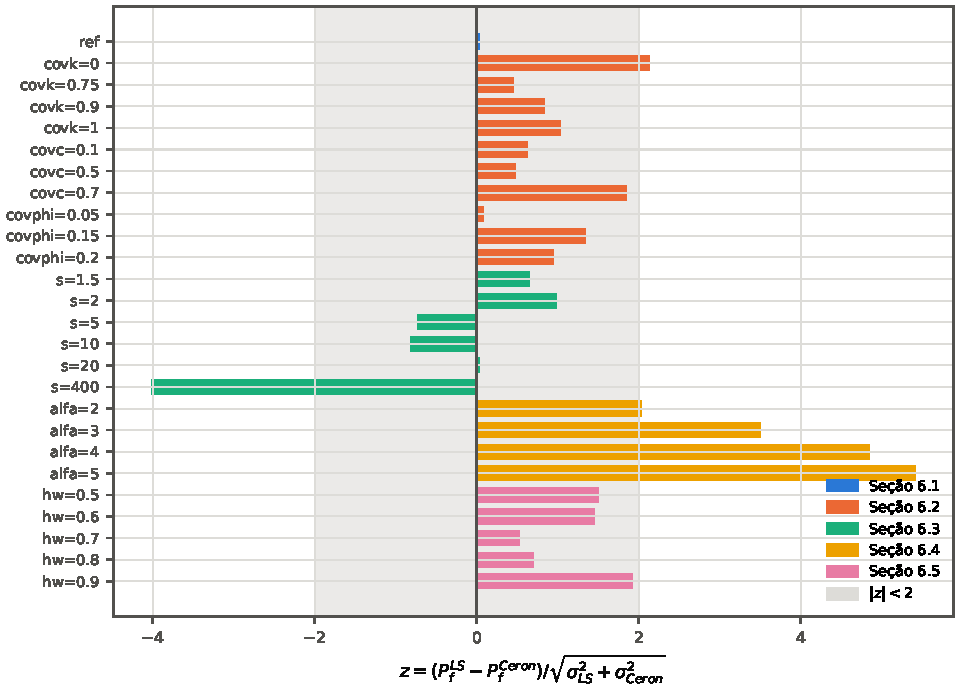
\includegraphics[width=0.85\linewidth]{figs/fig_z.pdf}
\caption{$z$ do LS contra o artigo em cada caso. A faixa cinza é $|z| < 2$.}\label{fig:z}
\end{figure}
\begin{itemize}
  \item \textbf{A água do artigo reproduz o artigo.} Com ela, o determinístico fica a $+0{,}4$ a $+1{,}2\,\%$ do
    artigo, a referência dá $\pfLSref\,\%$ contra $11{,}50\,\%$, e \nZdois{} dos \nCasos{} casos ficam a menos de dois
    desvios (\nZum{} a menos de um). A água antiga dava $\pfAntigaRef\,\%$ na referência e um efeito de $\alpha$ bem
    menor no determinístico.
  \item \textbf{O sinal de $z$ tem padrão} (Figura~\ref{fig:z}): quase todos os casos com variabilidade espacial
    ficam um pouco acima do artigo, e os de campo suave ($s \ge 5$), um pouco abaixo. É o que se espera de um MEF com
    mecanismo livre, que acha caminhos mais fracos que a família de espirais do artigo, somado a um viés de malha de
    $+0{,}8\,\%$ no $\Gamma$, que puxa a $P_f$ para baixo e passa a dominar quando o campo fica suave. Os casos estão
    pareados (os mesmos números aleatórios), então o padrão não é uma prova estatística.
  \item \textbf{A média de $\Gamma$ confirma a leitura:} com \nMCmin{} a \nMCmax{} realizações, a média do MC fica
    abaixo da do artigo em \nMuAbaixo{} dos \nMuTotal{} casos (de \muDifMinAll{} a \muDifMaxAll\,\%), embora o
    determinístico fique de +0,4 a +1,2\,\% acima. Na referência, a nossa média fica \muVsDetRef\,\% do nosso
    determinístico, e a do artigo, 1,3\,\% acima do dele: no MEF, a variabilidade espacial baixa a média de $\Gamma$,
    porque o mecanismo acha as zonas fracas; na família de espirais do artigo, não. Os casos estão pareados e o MC
    ainda é parcial, então isso é uma tendência, não um teste.
  \item \textbf{O que fica aberto:} a família $\alpha$ ($z$ de \zAlfaII{} a \zAlfaV) e o $s = 400$ ($z = \zSCD$),
    com os testes das Seções~\ref{sec:s} e \ref{sec:alfa}.
  \item \textbf{O método:} o LS chegou a $CoV \le 5\,\%$ em 22 dos 26 casos, com 110 a 1083 análises; dois ficaram
    em 5,0 e 5,1\,\%, e o $CoV(c) = 0{,}1$ e o $\alpha = 5$ pararam nas 600 linhas com 9,0 e 5,7\,\%. O FORM modal
    custou de 3 a 7 análises. O MC direto para $CoV = 5\,\%$ pediria $400(1 - P_f)/P_f$ análises: 3100 na referência
    e $\approx 28\,000$ com $\alpha = 4$.
  \item \textbf{O que falta rodar:}
    \begin{itemize}
      \item o MC pareado até 500 realizações por caso (rodando; este relatório se refaz com \texttt{gera.sh});
      \item $\alpha = 4$ com $CoV(k_v) = 0$ e o $\Gamma$ cinemático nas mesmas realizações do $\alpha = 4$;
      \item a malha: o $\Gamma$ com mais um nível (ou a extrapolação) na referência e em $s = 400$, e a integração em
        duas variáveis do $s = 400$.
    \end{itemize}
\end{itemize}


\begin{thebibliography}{9}
\bibitem{ceron2025} M.~Vargas Ceron, D.~L.~Cecílio, R.~V.~Linn, S.~Maghous. Stability analysis of slope subjected to
  seepage forces considering spatial variability of soil properties. \emph{International Journal for Numerical and
  Analytical Methods in Geomechanics}, 49(11):2459--2491, 2025. doi:10.1002/nag.3993.
\bibitem{hasofer1974} A.~M.~Hasofer, N.~C.~Lind. Exact and invariant second-moment code format. \emph{Journal of the
  Engineering Mechanics Division (ASCE)}, 100(1):111--121, 1974.
\bibitem{rackwitz1978} R.~Rackwitz, B.~Fiessler. Structural reliability under combined random load sequences.
  \emph{Computers \& Structures}, 9(5):489--494, 1978.
\bibitem{koutsourelakis2004} P.~S.~Koutsourelakis, H.~J.~Pradlwarter, G.~I.~Schuëller. Reliability of structures in
  high dimensions, part~I: algorithms and applications. \emph{Probabilistic Engineering Mechanics}, 19(4):409--417,
  2004. doi:10.1016/j.probengmech.2004.05.001.
\bibitem{clopper1934} C.~J.~Clopper, E.~S.~Pearson. The use of confidence or fiducial limits illustrated in the case of
  the binomial. \emph{Biometrika}, 26(4):404--413, 1934.
\bibitem{conover1999} W.~J.~Conover. \emph{Practical Nonparametric Statistics}. 3.\ ed. Wiley, 1999.
\bibitem{formulacao} Campos aleatórios e confiabilidade de taludes: as bases de Karhunen--Loève (analítica e Nyström),
  o FORM com gradiente modal (SRM e GIM) e o line sampling. Documento interno,
  \path{docs/confiabilidade_campos/formulacao/formulacao.pdf}, 2026.
\bibitem{contornos} Os contornos da água no rebaixamento e na chuva: Ceron (2025), o PZ e Rahardjo et al.\ (2007).
  Documento interno, \path{Projects/PlanoDeTrabalho/contornos_agua/relatorio_contornos.pdf}, 2026.
\bibitem{antigo} Exemplo da Seção~6 de Vargas Ceron et al.\ (2025) com a água permanente antiga: comparação.
  Relatório interno de 13/11/2026, \path{Projects/PlanoDeTrabalho/arquivo/2026-11-13_relatorio_ceron_agua_antiga.pdf}.
\end{thebibliography}

\appendix
\section{Arquivos e como refazer}
\begin{itemize}
  \item \textbf{A campanha:} \path{Projects/SlopeRandomFieldRefinement/cluster/ls_ceron_casos.sbatch}, com os casos em
    \path{casos_ls_ceron.txt}; saída no fermi em \path{$DATA/ceron_ls_casos}.
  \item \textbf{O download:} \path{cluster/baixar_ls_ceron.sh} (pede a senha) grava em
    \path{~/projects/runs/fermi_ceron_ls_casos} o resumo (\texttt{resumo\_ls\_ceron.py}) e as figuras do artigo
    (\texttt{figuras\_ls\_ceron.py}, em \path{Projects/SlopeRandomField/comparacao_ceron}).
  \item \textbf{Este relatório:} \texttt{gera.sh} roda o resumo e as figuras sobre o que já foi baixado, o
    \texttt{gera\_dados.py} (tabelas em \path{tab/}, números em \path{numeros.tex}, as Figs.~26, de $z$ e das raízes)
    e o \LaTeX.
  \item \textbf{A Fig.~26 do artigo} foi lida nos pixels das barras do PDF (página 2481): $c = 0{,}879$,
    $\varphi = 0{,}509$ e $k_v = -0{,}036$.
  \item \textbf{As colunas da água antiga} vêm do \path{estatisticas.json} do relatório de 13/11, no arquivo.
\end{itemize}
\end{document}
